The function \emph{prune\_example(x,y)} initially creates a decision tree for predicting the response \emph{y} from the input
values \emph{x}. In this case \emph{x} represents a vector of 100 x 45 our
example data and \emph{y} a vector of 100 x 1 labels for each of the training
examples.

Cost vectors for the tree are generated using resubstitution and 10-fold
cross-validation.

Resubstitution estimates an error rate over over a classifier constructed from
an entire sample. It is likely that this technique will not predict accuratly
the error rate, when exposed to new data.

For ten-fold cross validation the data is partitioned into 10 sets. With one
set being held for validation and the other 9 being used for training, this is
repeated 10 times using each set as the validation set. These error estimates are
combined to produce an overall over estimate. This is used to help identify
overfitting of the learning mechanism to the training data.

Once the level over pruning has been determined the tree is pruned with the
\emph{treeprune()} function. This helps to reduce the computational cost of
classification and may also help to remove a certain level of 'overfit'. Figure \ref{fig:pruning} plots the results of the validation techiques.

\begin{figure}[h]
    \centering
    \subfloat[Ten-fold cross-validation]{\label{fig:fig1}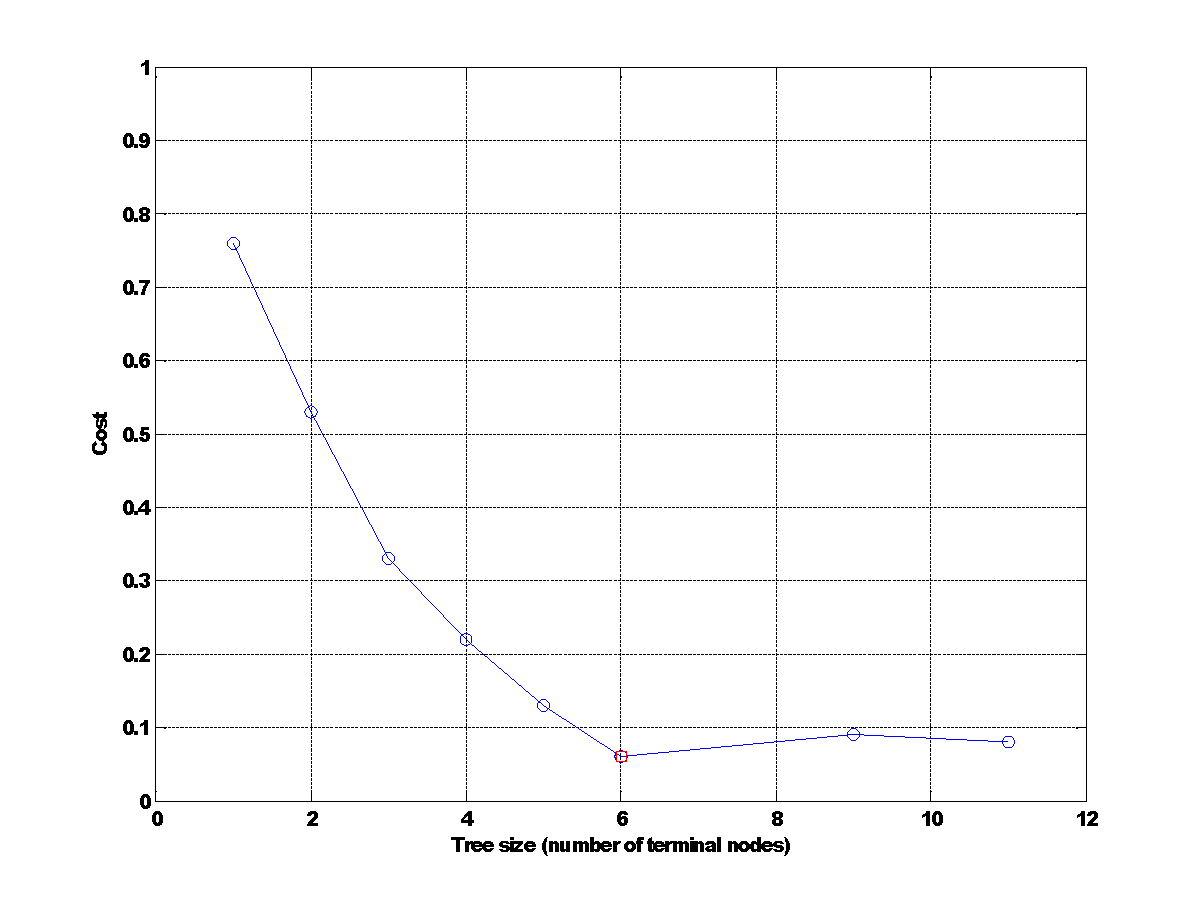
\includegraphics[width=0.5\textwidth]{fig1.pdf}}
    \subfloat[Resubstitution]{\label{fig:fig2}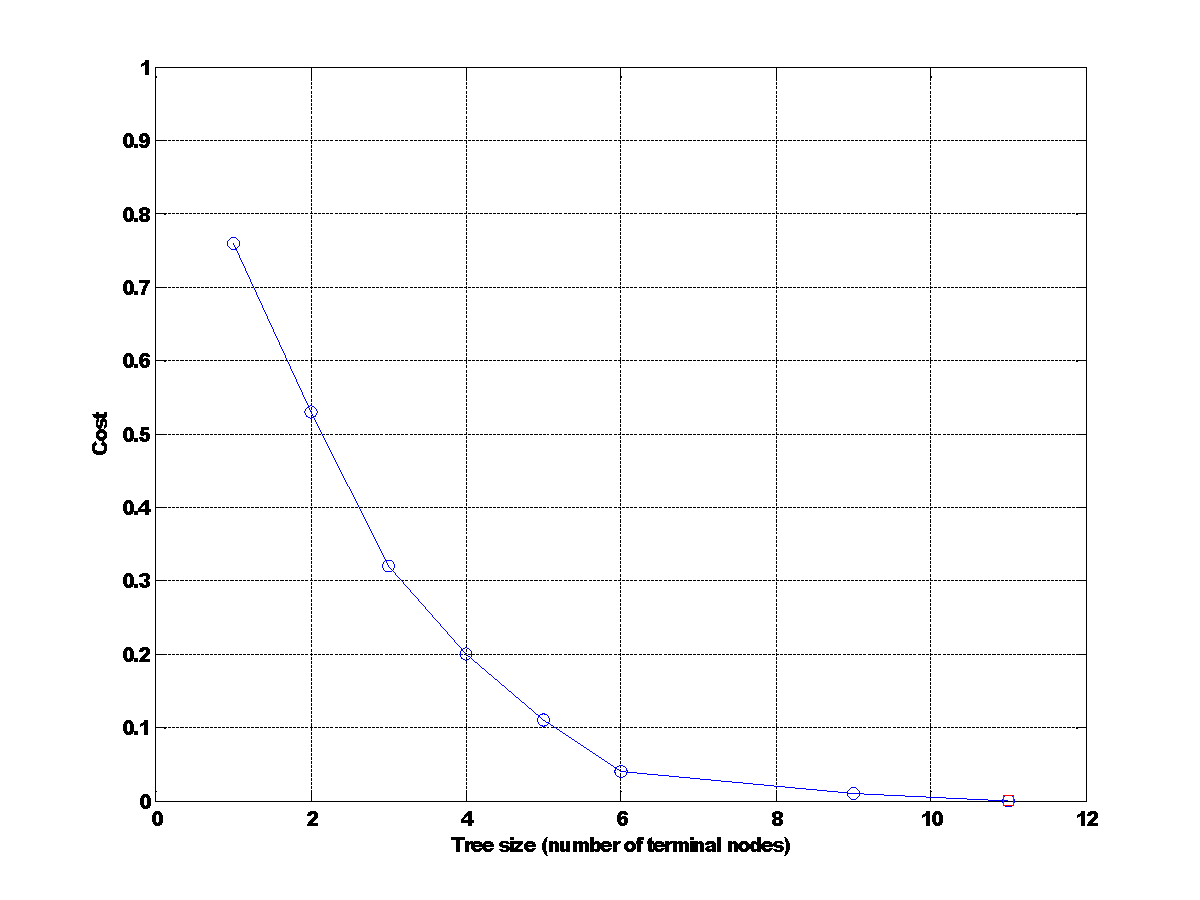
\includegraphics[width=0.5\textwidth]{fig2.pdf}}
    \caption{Pruning plots}
    \label{fig:pruning}
\end{figure}
